\documentclass{article}

\usepackage{booktabs}
\usepackage{tabularx}
\usepackage{graphicx}
\usepackage{geometry}
\usepackage{float}

%% Comments

\usepackage{color}

\newif\ifcomments\commentstrue %displays comments
%\newif\ifcomments\commentsfalse %so that comments do not display

\ifcomments
\newcommand{\authornote}[3]{\textcolor{#1}{[#3 ---#2]}}
\newcommand{\todo}[1]{\textcolor{red}{[TODO: #1]}}
\else
\newcommand{\authornote}[3]{}
\newcommand{\todo}[1]{}
\fi

\newcommand{\wss}[1]{\authornote{blue}{SS}{#1}} 
\newcommand{\plt}[1]{\authornote{magenta}{TPLT}{#1}} %For explanation of the template
\newcommand{\an}[1]{\authornote{cyan}{Author}{#1}}

%% Common Parts

\newcommand{\progname}{Software Engineering} % PUT YOUR PROGRAM NAME HERE
\newcommand{\authname}{Team \#13, ARC
    \\ Avanish, Ahluwalia
    \\ Russell, Davidson
    \\ Rafey, Malik
    \\ Abdul, Zulfiqar} % AUTHOR NAMES                  

\usepackage{hyperref}
    \hypersetup{colorlinks=true, linkcolor=blue, citecolor=blue, filecolor=blue,
                urlcolor=blue, unicode=false}
    \urlstyle{same}
                                


\title{Usability Testing\\\progname}

\author{\authname}

\date{}

\begin{document}

\maketitle

\newpage

\begin{table}[hp]
\caption{Revision History} \label{TblRevisionHistory}
\begin{tabularx}{\textwidth}{llX}
\toprule
\textbf{Date} & \textbf{Version} & \textbf{Change}\\
\midrule
2025-04-01 & 1.0 & Initial Version \\
\bottomrule
\end{tabularx}
\end{table}

~\newpage

\tableofcontents

~\newpage

\pagenumbering{arabic}

\section{Introduction}

To gain a better understanding of how usable the Realm app is, two usability surveys were conducted: one for Rev0 and one for Rev1. Having these done at different stages of development provides the team with a data-backed view on the success of tailoring the app based on user feedback. The results of the first survey were already published in the \textit{VnV Report}, but they will be shown again for comparison purposes. Using the most up-to-date data, future development steps will be outlined based on areas the require the most work from a user perspective.

\section{Survey}
The survey consists of six questions where participants rate on a scale of 1-5 how much they agree/disagree with a statement relating to their user experience. \\

\noindent The following statements were put forward and rated by the user on a scale from 1 (strongly disagree) to 5 (strongly agree):
\begin{enumerate}
    \item Navigation between interfaces is intuitive
    \item Placing objects in edit mode is easy
    \item Generating objects through prompts is easy
    \item It is easy to start a tour
    \item The app is generally satisfying to use
    \item Using the app distracts you from your surroundings
\end{enumerate}

\section{Results}
This section will analyze the results of the usability survey completed by users who were using the app for the first time.

~\newpage

\subsection{Rev0 Survey}

\newgeometry{left=2.5cm,bottom=0.1cm}
\begin{table}[H]
  \caption{\bf Results of Rev0 Usability Survey}
  \resizebox{6.5in}{!}{\begin{tabular}{|p{0.4\linewidth}|p{0.3\linewidth}|p{0.7\linewidth}|}
      \hline
      {\bfseries Statement}                         & {\bfseries Average Rating of Statement Accuracy / 5} & {\bfseries Analysis}                                                                                                                                                               \\
      \hline
      Navigation between interfaces is intuitive    & 3.833                                                & Most users found the navigation to be intuitive, although navigation seems to be the lowest rated aspect of the functional user experience                                         \\
      \hline
      Placing objects is easy                       & 3.917                                                & No ratings below a three and an average rating of "Agree" says that this was well received                                                                                         \\
      \hline
      Generating objects is easy                    & 3.917                                                & Again, no ratings below a three and an average rating of "Agree" indicates that the design works for most users                                                                    \\
      \hline
      It is easy to start a tour                    & 4.167                                                & A good indication that the touring experience was designed well                                                                                                                    \\
      \hline
      The app is generally satisfying to use        & 3.667                                                & This was the lowest rating of all our positive statements. We received relevant feedback on the non-uniform look and feel of the app making the app feel like a rushed development \\
      \hline
      Using the app distracts from the surroundings & 3.167                                                & More found the app distracting than not, but the results are somewhat inconclusive given the variance                                                                              \\
      \hline
    \end{tabular}}
  \label{table:US1}
\end{table}

\begin{figure}[H]
  \caption{Rev0 - "Navigation between interfaces is intuitive" statement ratings}
  \centerline{\includegraphics[scale=0.35]{./Survey_Images/Rev0/Q1.png}}
  \label{fig:StraightForward}
\end{figure}

\begin{figure}[H]
  \caption{Rev0 - "Placing objects is easy" statement ratings}
  \centerline{\includegraphics[scale=0.35]{./Survey_Images/Rev0/Q2.png}}
  \label{fig:Navigation}
\end{figure}

\begin{figure}[H]
  \caption{Rev0 - "Generating objects is easy" statement ratings}
  \centerline{\includegraphics[scale=0.35]{./Survey_Images/Rev0/Q3.png}}
  \label{fig:Detached}
\end{figure}

\begin{figure}[H]
  \caption{Rev0 - "It is easy to start a tour" statement ratings}
  \centerline{\includegraphics[scale=0.35]{./Survey_Images/Rev0/Q4.png}}
  \label{fig:RealWorld}
\end{figure}

\begin{figure}[H]
  \caption{Rev0 - "The app is generally satisfying to use" statement ratings}
  \centerline{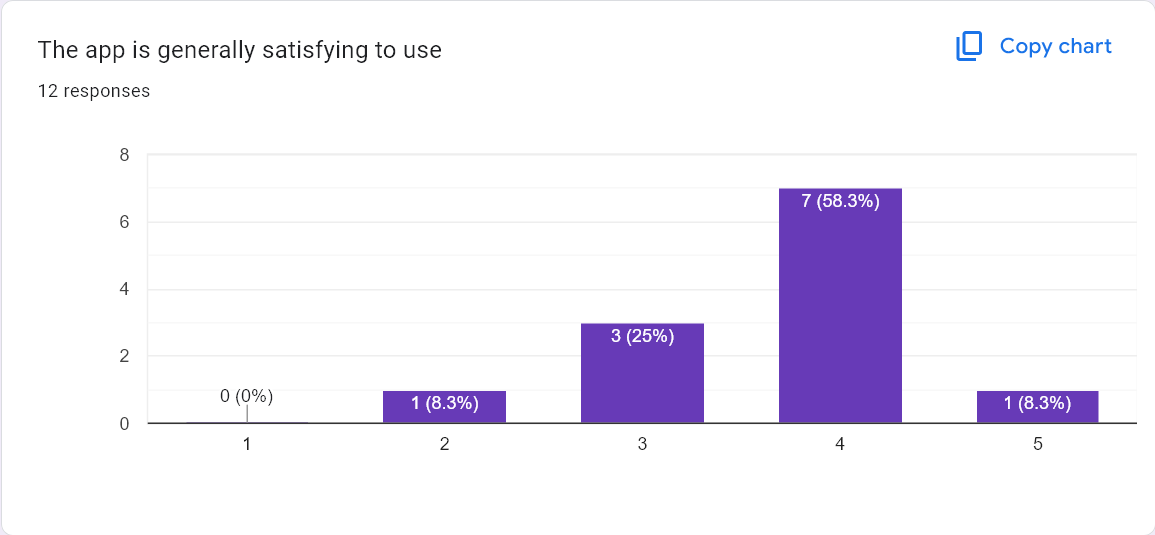
\includegraphics[scale=0.35]{./Survey_Images/Rev0/Q5.png}}
  \label{fig:Social}
\end{figure}

\begin{figure}[H]
  \caption{Rev0 - "Using the app distracts from the surroundings" statement ratings}
  \centerline{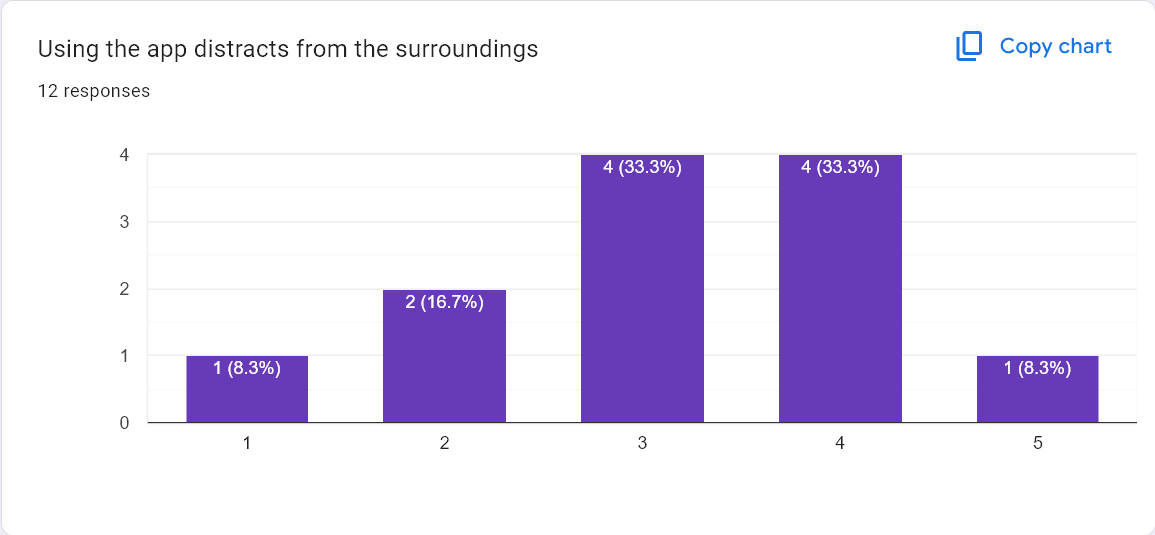
\includegraphics[scale=0.35]{./Survey_Images/Rev0/Q6.png}}
  \label{fig:Enjoy}
\end{figure}

~\newpage

\subsection{Rev1 Survey}

\newgeometry{left=2.5cm,bottom=0.1cm}
\begin{table}[H]
  \caption{\bf Results of Rev1 Usability Survey}
  \resizebox{6.5in}{!}{\begin{tabular}{|p{0.4\linewidth}|p{0.3\linewidth}|p{0.7\linewidth}|}
      \hline
      {\bfseries Statement}                         & {\bfseries Average Rating of Statement Accuracy / 5} & {\bfseries Analysis}                                                                                                                                                               \\
      \hline
      Navigation between interfaces is intuitive         & 4.889                                                & This was the second highest rated user experience. Users seemed to be able to navigate without a problem.                                        \\
      \hline
      Placing objects in edit mode is easy               & 4.000                                                & Most users generally agree with this statement with many strongly agreeing. There was some more variance in the response to this statement probably due to the many potential conditions objects can be placed under.                                                                                         \\
      \hline
      Generating objects through prompts is easy         & 4.556                                                & Most users strongly agree that prompt generation is easy.                                                                    \\
      \hline
      It is easy to start a tour                         & 5.000                                                & This was the highest rated user experience. It makes sense because it is only two simple clicks from the home page to start a tour.                                                                                                                    \\
      \hline
      The app is generally satisfying to use             & 3.889                                                & Most users tended to agree that the app was satisfying overall but most still had feedback on places where it could be improved. \\
      \hline
      Using the app distracts you from your surroundings & 2.556                                                & There was much variance in rating this statement maybe due to the vagueness of the statement itself. Most users disagreed that the app distracts them from their surroundings.                                                                            \\
      \hline
    \end{tabular}}
  \label{table:US1}
\end{table}

\begin{figure}[H]
  \caption{Rev1 - "Navigation between interfaces is intuitive" statement ratings}
  \centerline{\includegraphics[scale=0.75]{./Survey_Images/Rev1/Q1.png}}
  \label{fig:StraightForward}
\end{figure}

\begin{figure}[H]
  \caption{Rev1 - "Placing objects in edit mode is easy" statement ratings}
  \centerline{\includegraphics[scale=0.75]{./Survey_Images/Rev1/Q2.png}}
  \label{fig:Navigation}
\end{figure}

\begin{figure}[H]
  \caption{Rev1 - "Generating objects through prompts is easy" statement ratings}
  \centerline{\includegraphics[scale=0.75]{./Survey_Images/Rev1/Q3.png}}
  \label{fig:Detached}
\end{figure}

\begin{figure}[H]
  \caption{Rev1 - "It is easy to start a tour" statement ratings}
  \centerline{\includegraphics[scale=0.75]{./Survey_Images/Rev1/Q4.png}}
  \label{fig:RealWorld}
\end{figure}

\begin{figure}[H]
  \caption{Rev1 - "The app is generally satisfying to use" statement ratings}
  \centerline{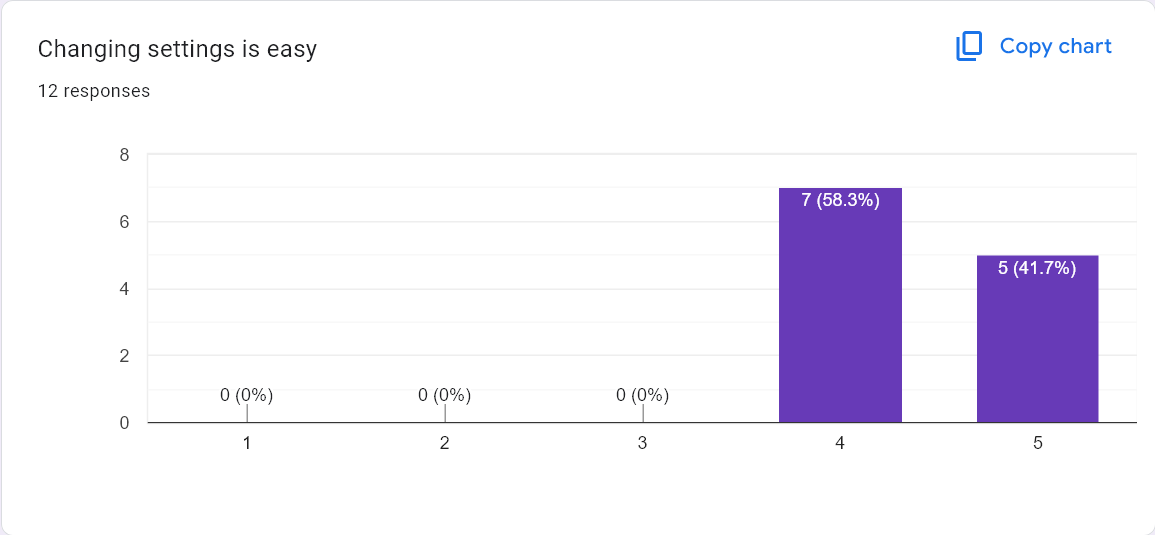
\includegraphics[scale=0.75]{./Survey_Images/Rev1/Q5.png}}
  \label{fig:Social}
\end{figure}

\begin{figure}[H]
  \caption{Rev1 - "Using the app distracts you from your surroundings" statement ratings}
  \centerline{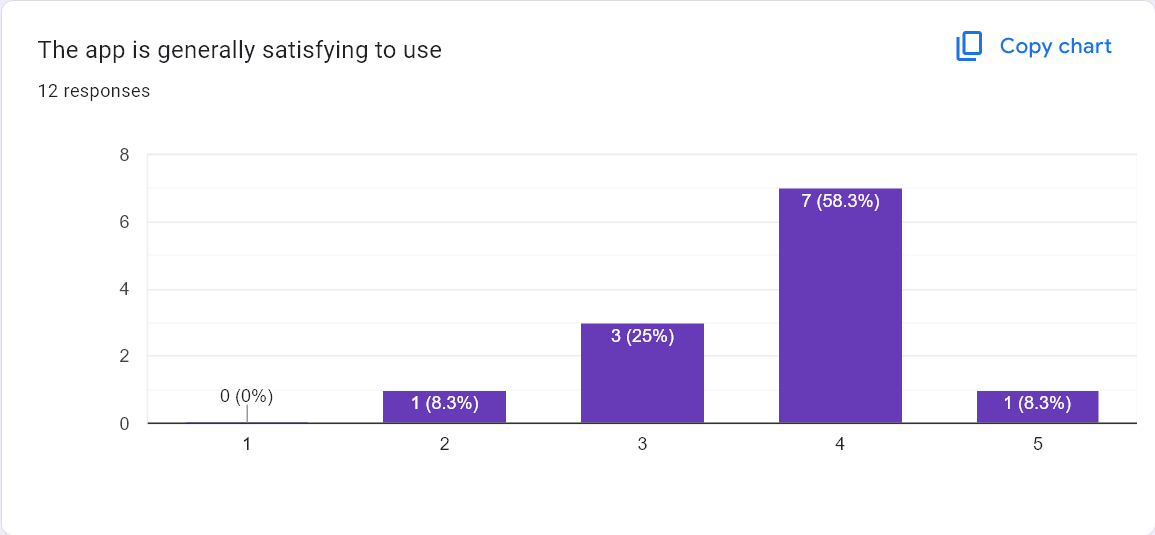
\includegraphics[scale=0.75]{./Survey_Images/Rev1/Q6.png}}
  \label{fig:Enjoy}
\end{figure}

\subsection{Comparison}
For each answer a comparison of the results will be conducted.

\begin{enumerate}
    \item \textit{Navigation between interfaces is intuitive}\\
    Since Rev0, much effort was put into the app user interface flow. This seems to have translated into increased user satisfaction in Rev1 with almost everyone liking it.
    \item \textit{Placing objects in edit mode is easy}\\
    The AR object placement flow did not change much between Rev0 and Rev1 so the similar results seems to track.
    \item \textit{Generating objects through prompts is easy}\\
    With the overall app UI improvements, also came improvements to the prompt generation screen which users seem to think is easy to use in Rev1.
    \item \textit{It is easy to start a tour}\\
    The app home screen now has a list of tours a user can choose from and preview. From here, they can start the tour. It only takes two button presses, so all users found this very easy.
    \item \textit{The app is generally satisfying to use}\\
    Most people liked the app for the most part in both Rev0 and Rev1 though it seems the rating went slightly down in Rev1.
    \item \textit{Using the app distracts you from your surroundings}\\
    This statement is relatively vague so that could account from the wide spread of ratings in both Rev0 and Rev1. Rev1 users found it less distracting likely due to the hiding of AR virtual planes in tour viewing mode.
\end{enumerate}

\section{Conclusion}
Through both of the usability tests conducted, users generally liked the app, and it seems they liked it even more after the changes were made to the app UI. There were still quite a few suggestions for improvements and new features that could be made in the future. These include more visual queues when going through the object placement steps and a more robust help feature for users who want to learn more about a specific feature.

\end{document}